\documentclass[tikz,border=4pt]{standalone}
\usepackage[utf8]{inputenc}
\usepackage[T1]{fontenc}
\usepackage{helvet}
\renewcommand{\familydefault}{\sfdefault}
\usetikzlibrary{arrows.meta,shapes.geometric,positioning}
\begin{document}
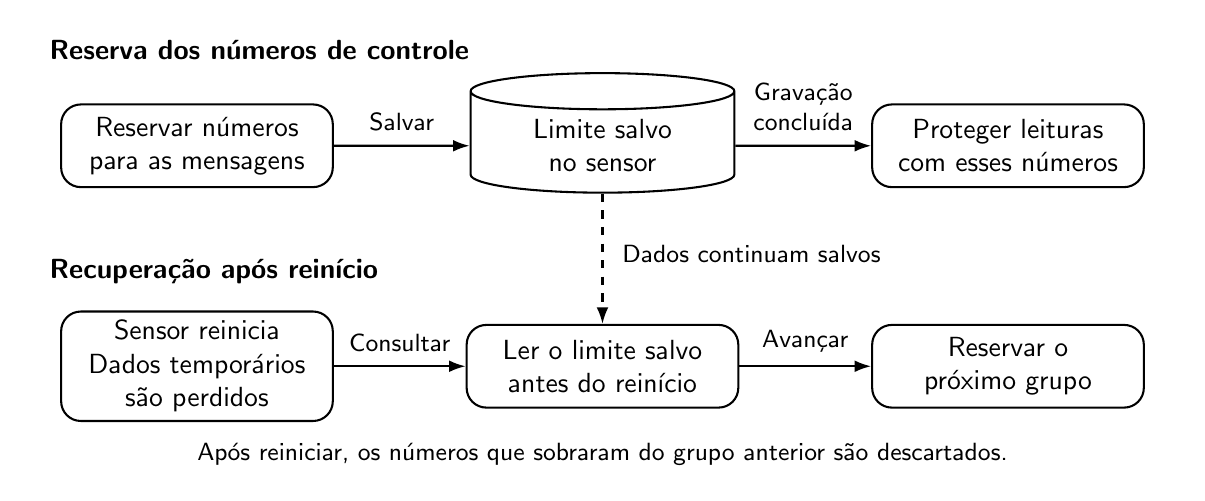
\begin{tikzpicture}[
  font=\sffamily\fontsize{10}{12}\selectfont,
  line width=0.75pt,
  flow/.style={-{Latex[length=2.1mm,width=1.5mm]}},
  block/.style={draw=black,fill=white,rounded corners=2.5mm,
    minimum width=3.45cm,minimum height=1.05cm,align=center},
  label/.style={font=\sffamily\fontsize{9}{11}\selectfont,align=center,fill=white,inner sep=2pt}
]
\path[use as bounding box] (0,-0.05) rectangle (14.6,5.6);

\node[anchor=west,font=\bfseries] at (0.15,5.32) {Reserva dos números de controle};
\node[block] (reserve) at (2.15,4.10)
  {Reservar números\\para as mensagens};
\node[draw=black,fill=white,cylinder,shape border rotate=90,aspect=0.23,
  minimum width=3.35cm,minimum height=1.35cm,align=center] (journal) at (7.30,4.10)
  {Limite salvo\\no sensor};
\node[block] (use) at (12.45,4.10)
  {Proteger leituras\\com esses números};

\draw[flow] (reserve.east) -- node[label,above=3pt] {Salvar} (journal.west);
\draw[flow] (journal.east) -- node[label,above=3pt] {Gravação\\concluída} (use.west);

\node[anchor=west,font=\bfseries] at (0.15,2.50) {Recuperação após reinício};
\node[block] (restart) at (2.15,1.30)
  {Sensor reinicia\\Dados temporários\\são perdidos};
\node[block] (recover) at (7.30,1.30)
  {Ler o limite salvo\\antes do reinício};
\node[block] (next) at (12.45,1.30)
  {Reservar o\\próximo grupo};

\draw[flow] (restart.east) -- node[label,above=3pt] {Consultar} (recover.west);
\draw[flow] (recover.east) -- node[label,above=3pt] {Avançar} (next.west);
\draw[flow,dashed] (journal.south) -- (recover.north);
\node[label,anchor=west] at (7.47,2.73) {Dados continuam salvos};

\node[align=center,font=\sffamily\fontsize{9}{11}\selectfont] at (7.30,0.18)
  {Após reiniciar, os números que sobraram do grupo anterior são descartados.};
\end{tikzpicture}
\end{document}
